\defChapterTarget[ArchitecturalDesign]{Architectural design}
    \section{\textit{Overview}: High-level components and their interaction}
    The whole software that will become the main core of the SafeStreets
    initiative will be developed as a distributed application, which means that
    the software will be executed (or run) on multiple devices within a network.
    It will have a three-layers logic and be divided as following:
    \begin{itemize}
        \item \textbf{P}: The \textbf{\emph{presentation}} layer will handle all
        \textit{incoming} (\textit{and outcoming}) relations with the customers
        \item \textbf{A}: The \textbf{\emph{application}} layer will work as a
        "man in the middle" between the \textbf{P}resentation layer and the
        \textbf{D}atabase layer and will hold all the needed logic for the
        software to correctly work;
        \item \textbf{D}: The \textbf{\emph{database}} layer will be needed in
        order to store and manage all needed (and requested) information of the
        initiative;
    \end{itemize}
    Each and every one of the layers the architecture will be composed by a
    (group of) machines. By doing this, it is meant to provide, to each layer,
    its own dedicated hardware, for either scalability, failure handling and
    flexibility reasons.\\
    The following image shows the high-level architecture of the system without
    providing any detail of the components which will form the structure of the
    software itself, which will be tackled later in this document.
    
    \begin{figure}[H]
        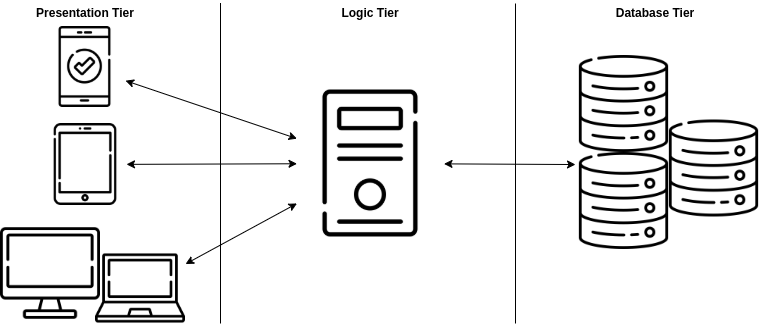
\includegraphics[scale=0.45]{dd/resources/images/HighLevelStructure.png}
        \caption{High-level architecture}        
    \end{figure}
 
    The introduction of the \textbf{P}resentation layer has been considered in
    order to allow a thin client architecture and let less performing devices
    access SafeStreets initiative and give a smoother feeling when using either
    the mobile or web version of the software. By doing so, this allows also for
    an high reusability of the code, since the logic is all implemented in the
    single \textbf{A}pplication layer, which allows different devices to access
    the same logic. The latter is the only tier which deals with two other tiers
    at the same time and is in charge of accessing data from the
    \textbf{D}atabase layer and pass it to the clients back and forth. In
    addition, the \emph{man in the middle} communicates with the Data tier
    synchronously when it comes to access the needed data, but asynchronously
    when storing and writing actions are required.\\
    \\
    The software will exploit a \textbf{P}latform \textbf{a}s \textbf{a}
    \textbf{S}ervice (\textbf{\emph{PaaS}}) provided by
    Amazon\textsuperscript{\textcopyright}. It has been chosen to create a
    \textbf{V}\textbf{P}\textbf{C} in order to attend the requirements stated in
    section 3.5 \emph{"Software System Attributes"} of the RASD. This will help
    also to augment the system scalability and improve the perfomances, as well
    as the reliability and security of the information stored in the system. \\
    The system is going to be modeled on a \emph{scale out} architecture: this
    will be improve the performance, as well as the failure management, by
    replicating nodes. This kind of architecture has been chosen, instead of a
    scale up architecture, as the latter is not suitable for a system thatplans
    to be eventually expanded and furtherly serve more and more customers. It
    comes without saying that the chosen kind of architecture will require the
    implementation of a \emph{load-balancing system} as well as a
    \emph{\textbf{S}hared \textbf{D}isk \textbf{C}onfiguration} (\textbf{SDC})
    in order to let all hardware write and read the same information at any
    moment. The latter has been chosen over a Shared Memory Configuration as it
    provides a certain degree of fault tolerance and does not create a
    bottleneck on the memory bus.\\
    Furthermore, in order to comply to the correct chain of custody that the
    system requires and to protect all sensible information of all customers,
    the installation of a proper \textbf{D}e\textbf{M}ilitarized \textbf{Z}one
    (\textbf{\emph{DMZ}}) is needed. This is accomplished by a series of
    firewalls created around the core tier of the software, the
    \emph{Application Tier}, the one that, if compromised by malicious users,
    could provide access to both other layers.\\ 
    \\ 
    The following image shows a detailed representation of the concepts above
    explained. Thanks to the decision of exploiting
    Amazon\textsuperscript{\textcopyright}'s services and its VPC, all the above
    mentioned architectural characteristics are automatically implemented, as
    the whole service is customizable and easily implementable.

    \begin{figure}[H]
        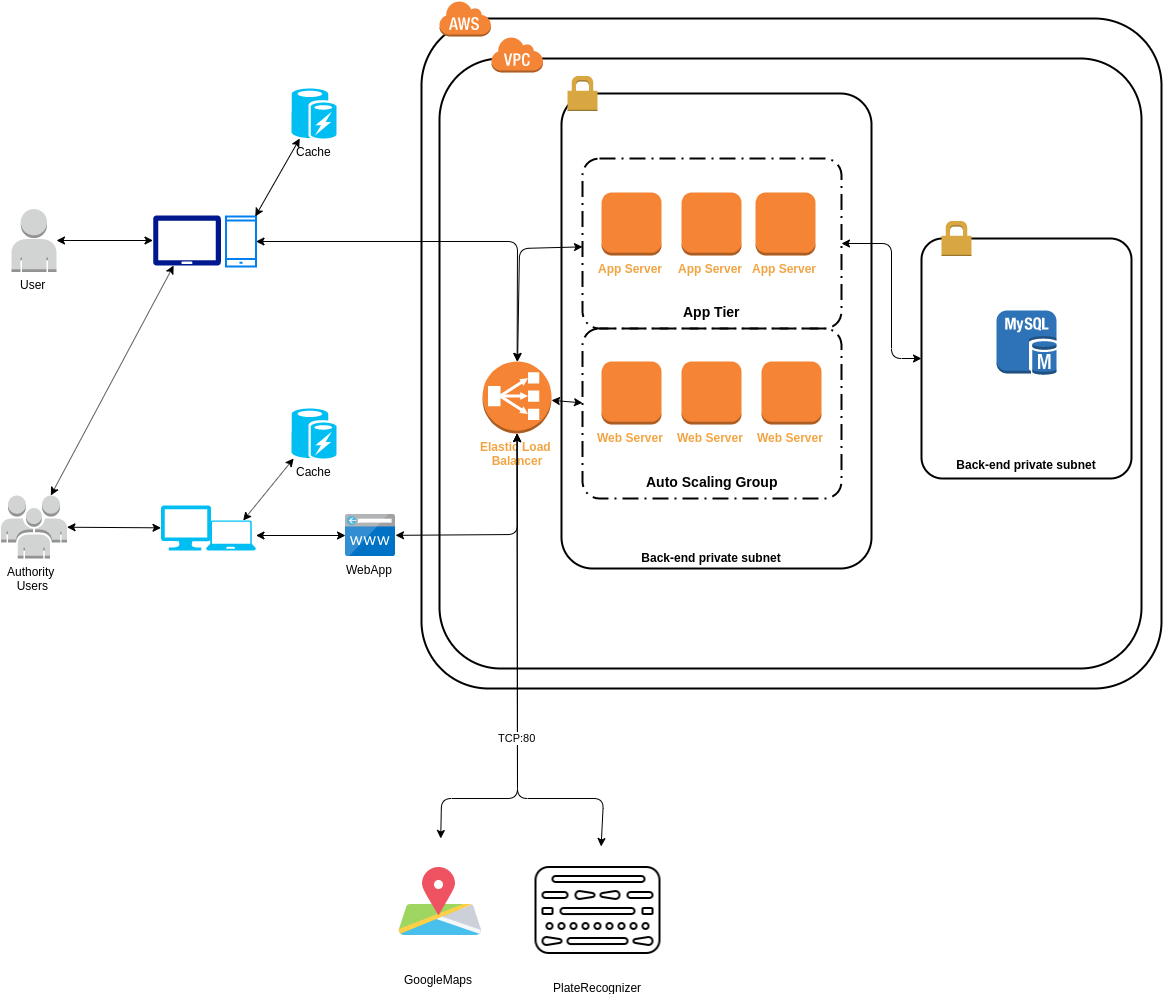
\includegraphics[scale=0.3]{dd/resources/images/ArchitecturalStructure.png}
        \caption{Architectural structure} 
    \end{figure}

    It is easily noticeable that there is no mention of the photo forensic
    software (\emph{Ghiro, per instance}) as this general architecture focuses
    on the software itself. Any additional photo forensic software, like the one
    proposed, has to be considered part of the "package" sold, but not needed to
    be developed as an already functioning software has been chosen. The sole
    purpose of SafeStreets is to ensure that the program is actually used and
    allow an automatic redirection to it. 

    \section{Component view}
    \begin{figure}[H]
        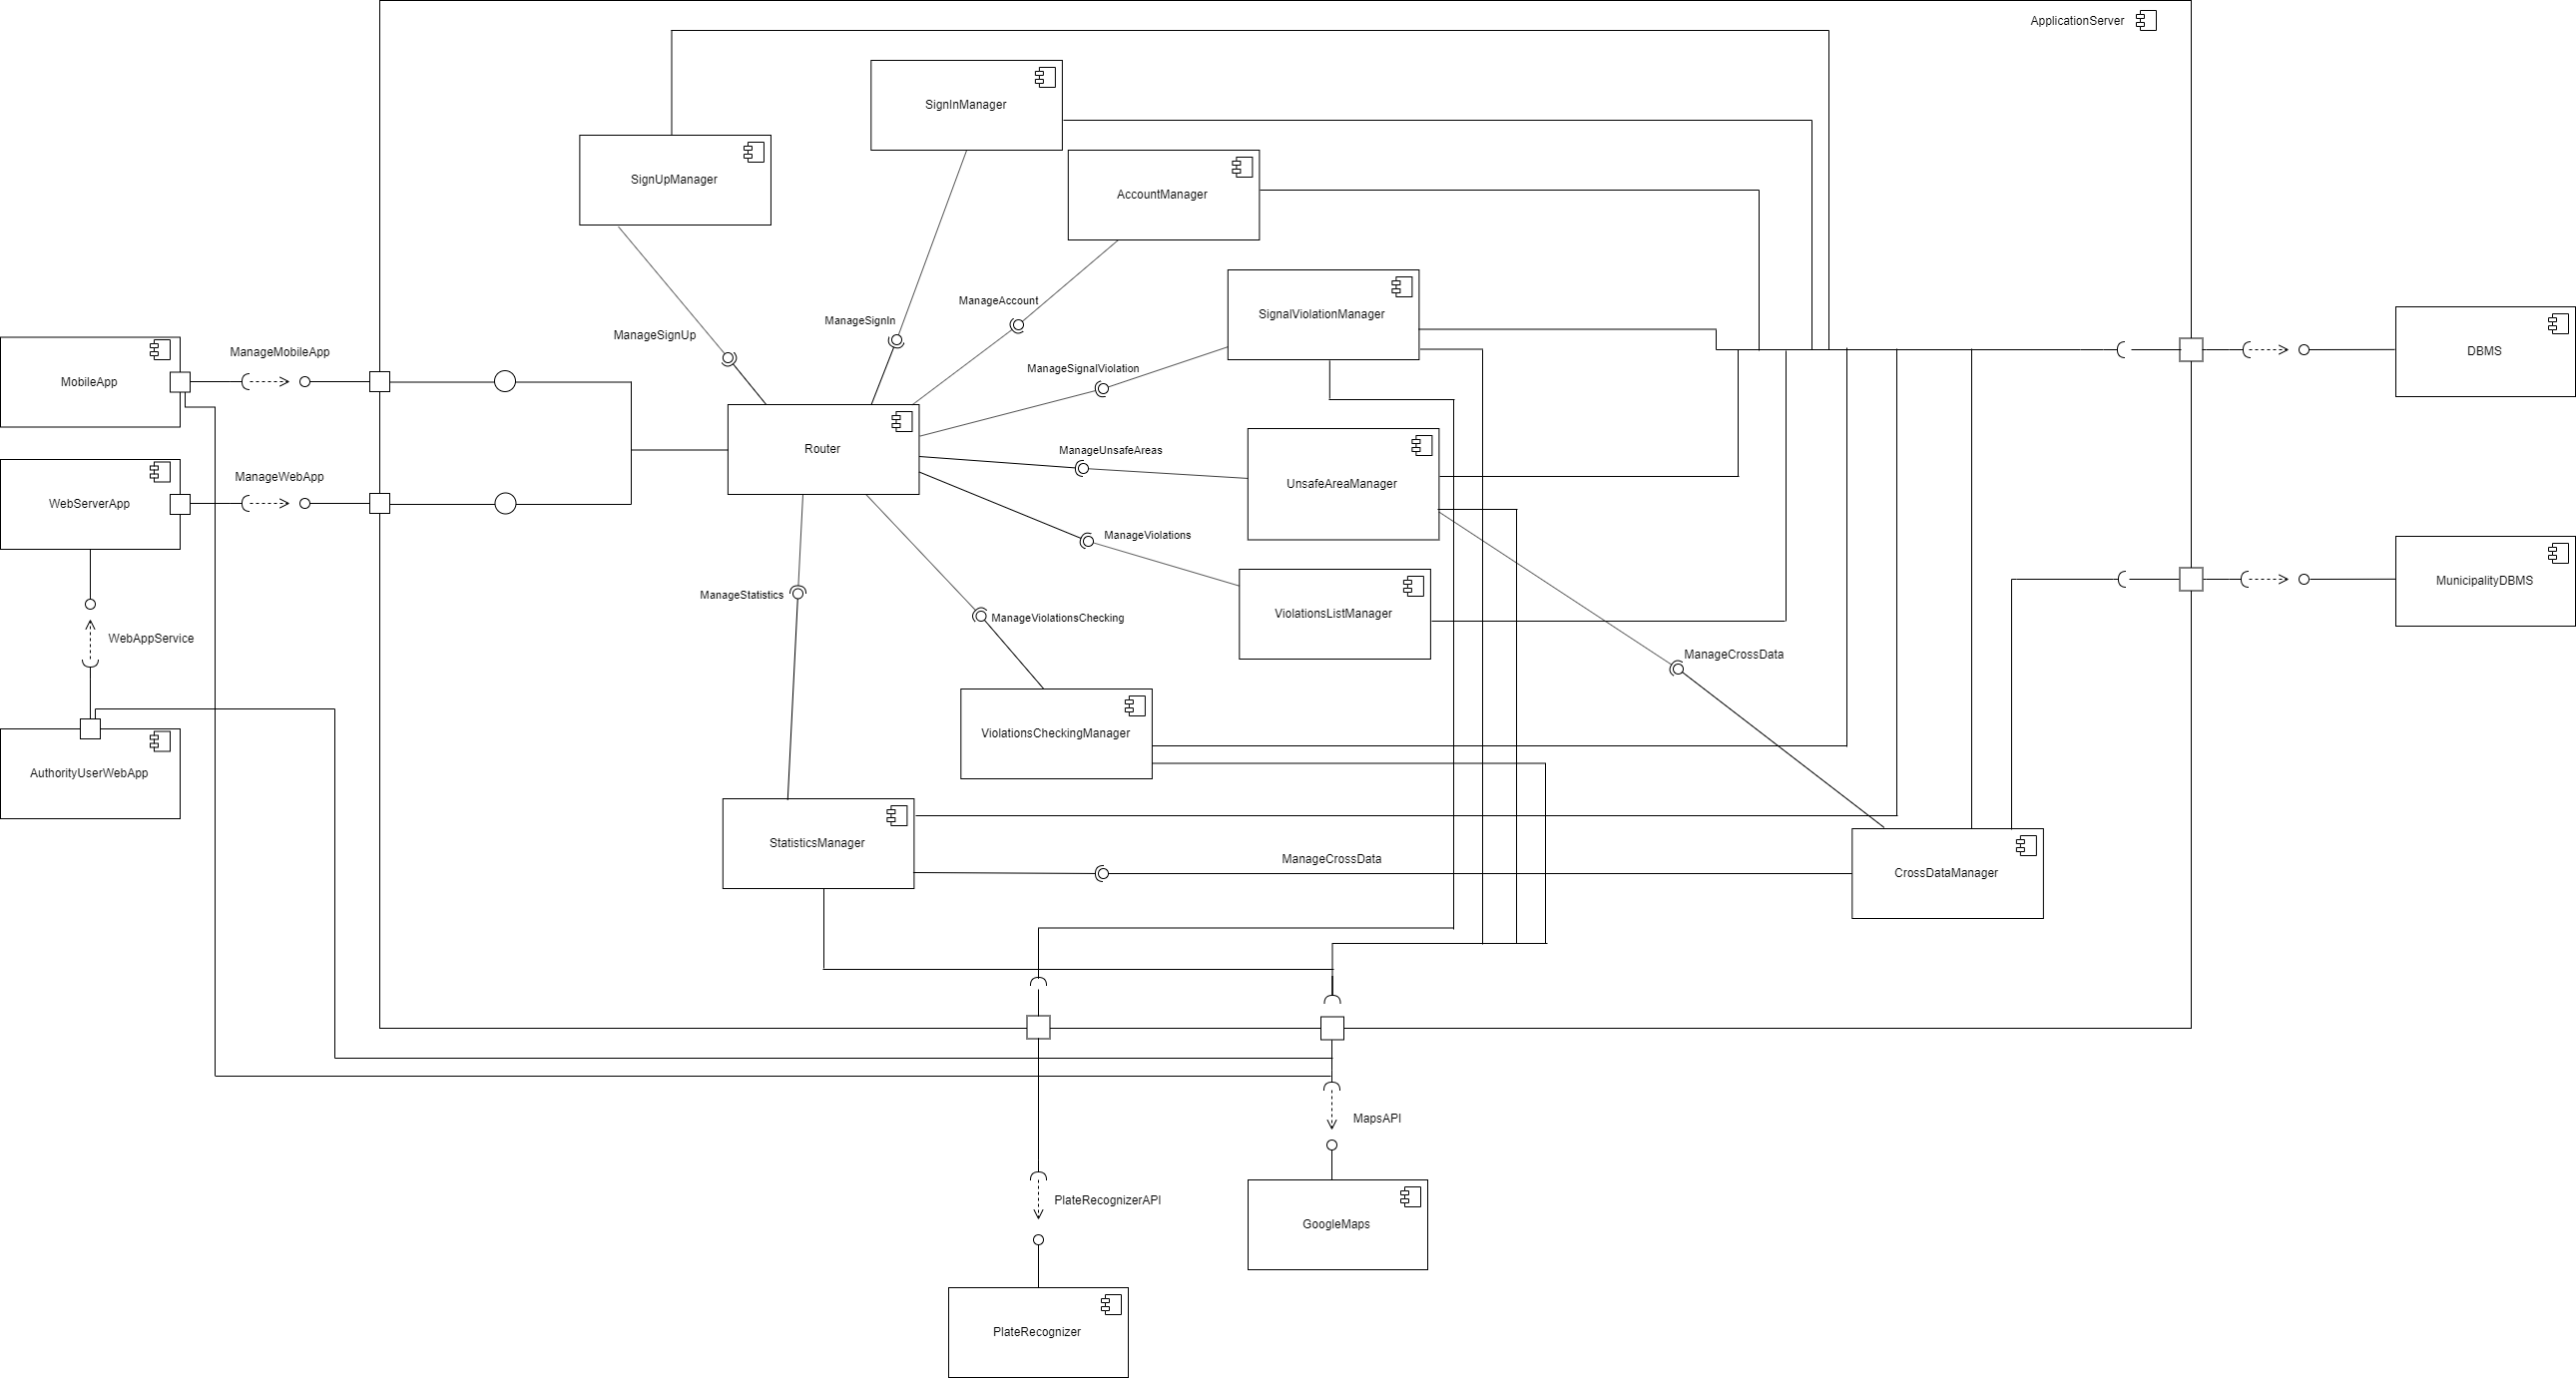
\includegraphics[scale=0.19,angle=90]{dd/resources/images/ComponentDiagram.png}
        \caption{Component Diagram}        
    \end{figure}
    \begin{itemize}
        \item \textbf{Router}:it manages messages and function calls coming from
        other subsystems in order to pass the data to the correct element of the
        system. It eventually calls the correspondent method/function on it.
        Furthermore, the router is partitioned according to the type of the
        interacting components because of the different functionalities. 
        \item \textbf{SignUpManager}: this component provides all the procedures
        to allow customers to register to SafeStreets. Obviously, this
        components has also to interact with the DBMS to store the registration
        data and to run a check about the chosen email, password and
        AuthoritiesID or fiscal code.
        \item \textbf{SignInManager}: it contains all the logic devoted to the
        authentication of the customers. It check the authentication parameters
        using the data stored on the DBMS.
        \item \textbf{AccountManager}: this component provides all the
        procedures to manage the account
        \item \textbf{SignalViolationManager}: it deals with the signalations of
        violations made by the users. This component has to verify that all the
        inserted data are correct and if not has to immediately ask the user to
        provide more information.
        \item \textbf{UnsafeAreasManager}: this component provides all the users
        the possibility to see the unsafe areas. It receives all the information
        from the DBMS.
        \item \textbf{ViolationsListManager}: with this component the user can
        see all the violations he/she has reported. The authority user can see
        all the violations reported in his/her area.
        \item \textbf{ViolationsCheckingManager}: this component provides the
        authority user the ability to check che violations.
        \item \textbf{StatisticsManager}: this component provides the authority
        user the possibility to see all the statistic generated crossing the
        data on violations. 
        \item \textbf{CrossDataManager}: it crosses data from SafeStreets
        database and from the municipality database to generate the statistics
        and the unsafe areas.
    \end{itemize}    
    \section{Deployment view}
    The following image is a deployment diagram which represents the
    architecture of the system as distribution(deployment) of software artifacts
    to deployment targets(node). Artifacts represents elements obtained with a
    development process. Nodes can represent either hardware or software environments.
    \begin{figure}[H]
        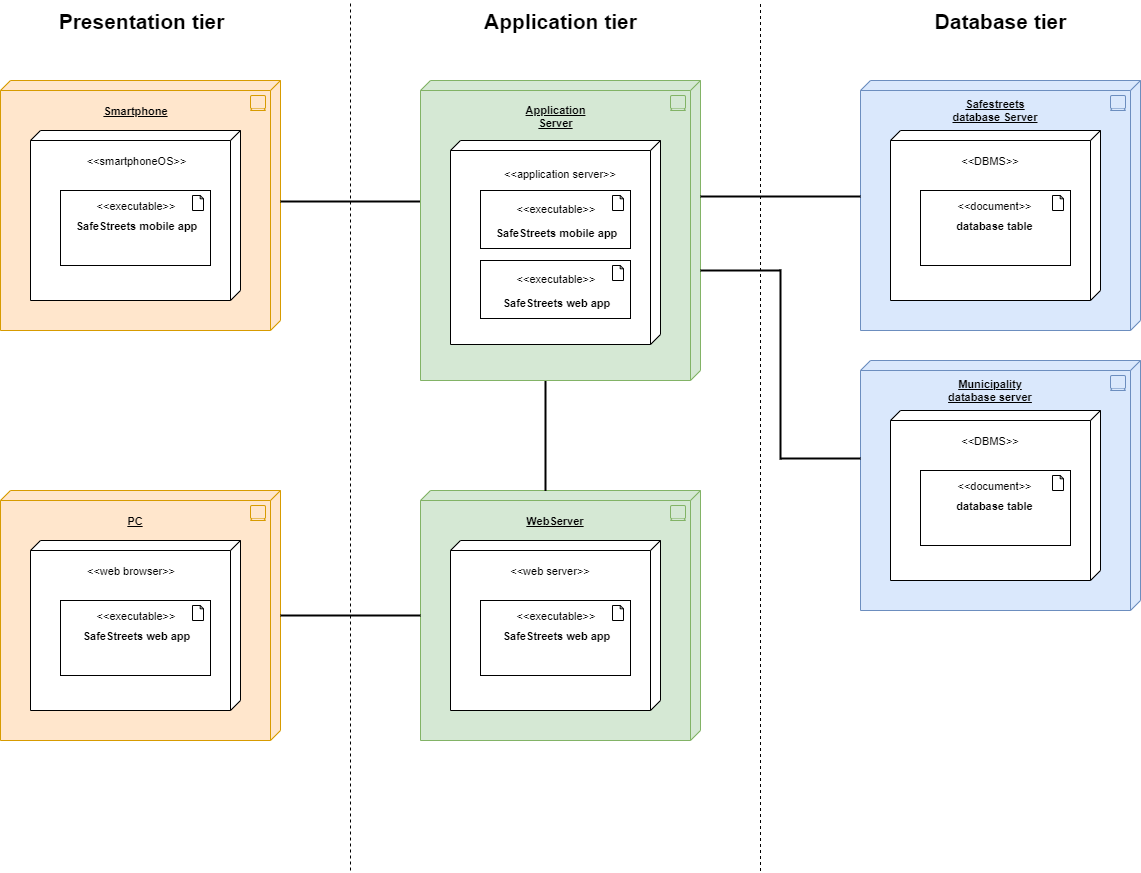
\includegraphics[scale=0.35]{dd/resources/images/DeploymentDiagram.png}
        \caption{Deployment view}        
    \end{figure}
    The three tiers contain:
    \begin{itemize}
        \item \textbf{Presentation tier}: in this tier the presentation logic is
        deployed. Users are provided with a mobile application on their mobile
        devices and authority users are provide with both a mobile application
        and a web application accessible from a common browser. The mobile
        application must be developed for most of the devices (both iOS and
        Android version). Both user and authority user ask to communicate to the
        application server in order to retrieve data, signal a violation, check
        violations or unsafe areas.
        \item \textbf{Application tier}: in this thier the application logic is
        deployed. The application server allows the mobile application and the
        web application to access data stored into the SafeStreets database. The
        application server also implements the business logic and handles the
        requests. The mobile application directly addresses the application
        server. The web server allow authority users to use SafeStreets
        services. If it can't provide some information it forwards the requests
        to the application server.
        \item \textbf{Database tier}: in this tier data access must be deployed.
        The application has to handle data both on SafeStreets database and on
        the municipality database for cross references.
    \end{itemize}    
    \section{Run-time view}
        \subsection{Synchronization}
        \subsection{Request data regarding a group of people}
        \subsection{Request data regarding a particular user by providing his/her UUID}
    \section{Component interface}
    \section{Selected architectural styles and patterns}  
    The architecture of SafeStreets is multilayered, composed of three tiers:
    \begin{itemize}
        \item \textbf{Presentation layer}: is used to present the data in a way
        that the user can understand. It enables the usage of the services
        offered to the user. The presentation layer of the the users is the
        smartphone and for authority users are both the smartphone and the browser.
        \item \textbf{Application layer}: is used to coordinate the application.
        It receives and computes the requests send by the presentation layer and
        it also interacts with the database.
        \item \textbf{Database layer}: stores the information provided by the
        application layer. The information is also passed back to the
        application tier for processing.
    \end{itemize}    
    Three tier architecture is very useful because it allows to change or upgrade
    one of the three tiers without any problem and so it makes the system more
    flexible and reusable. Furthermore it makes the system safer because it
    separates the access to data from the other layers.
  
        \subsection{Design Patterns}
            \subsubsection*{Model View Controller (MVC)}
            \begin{figure}[H]
                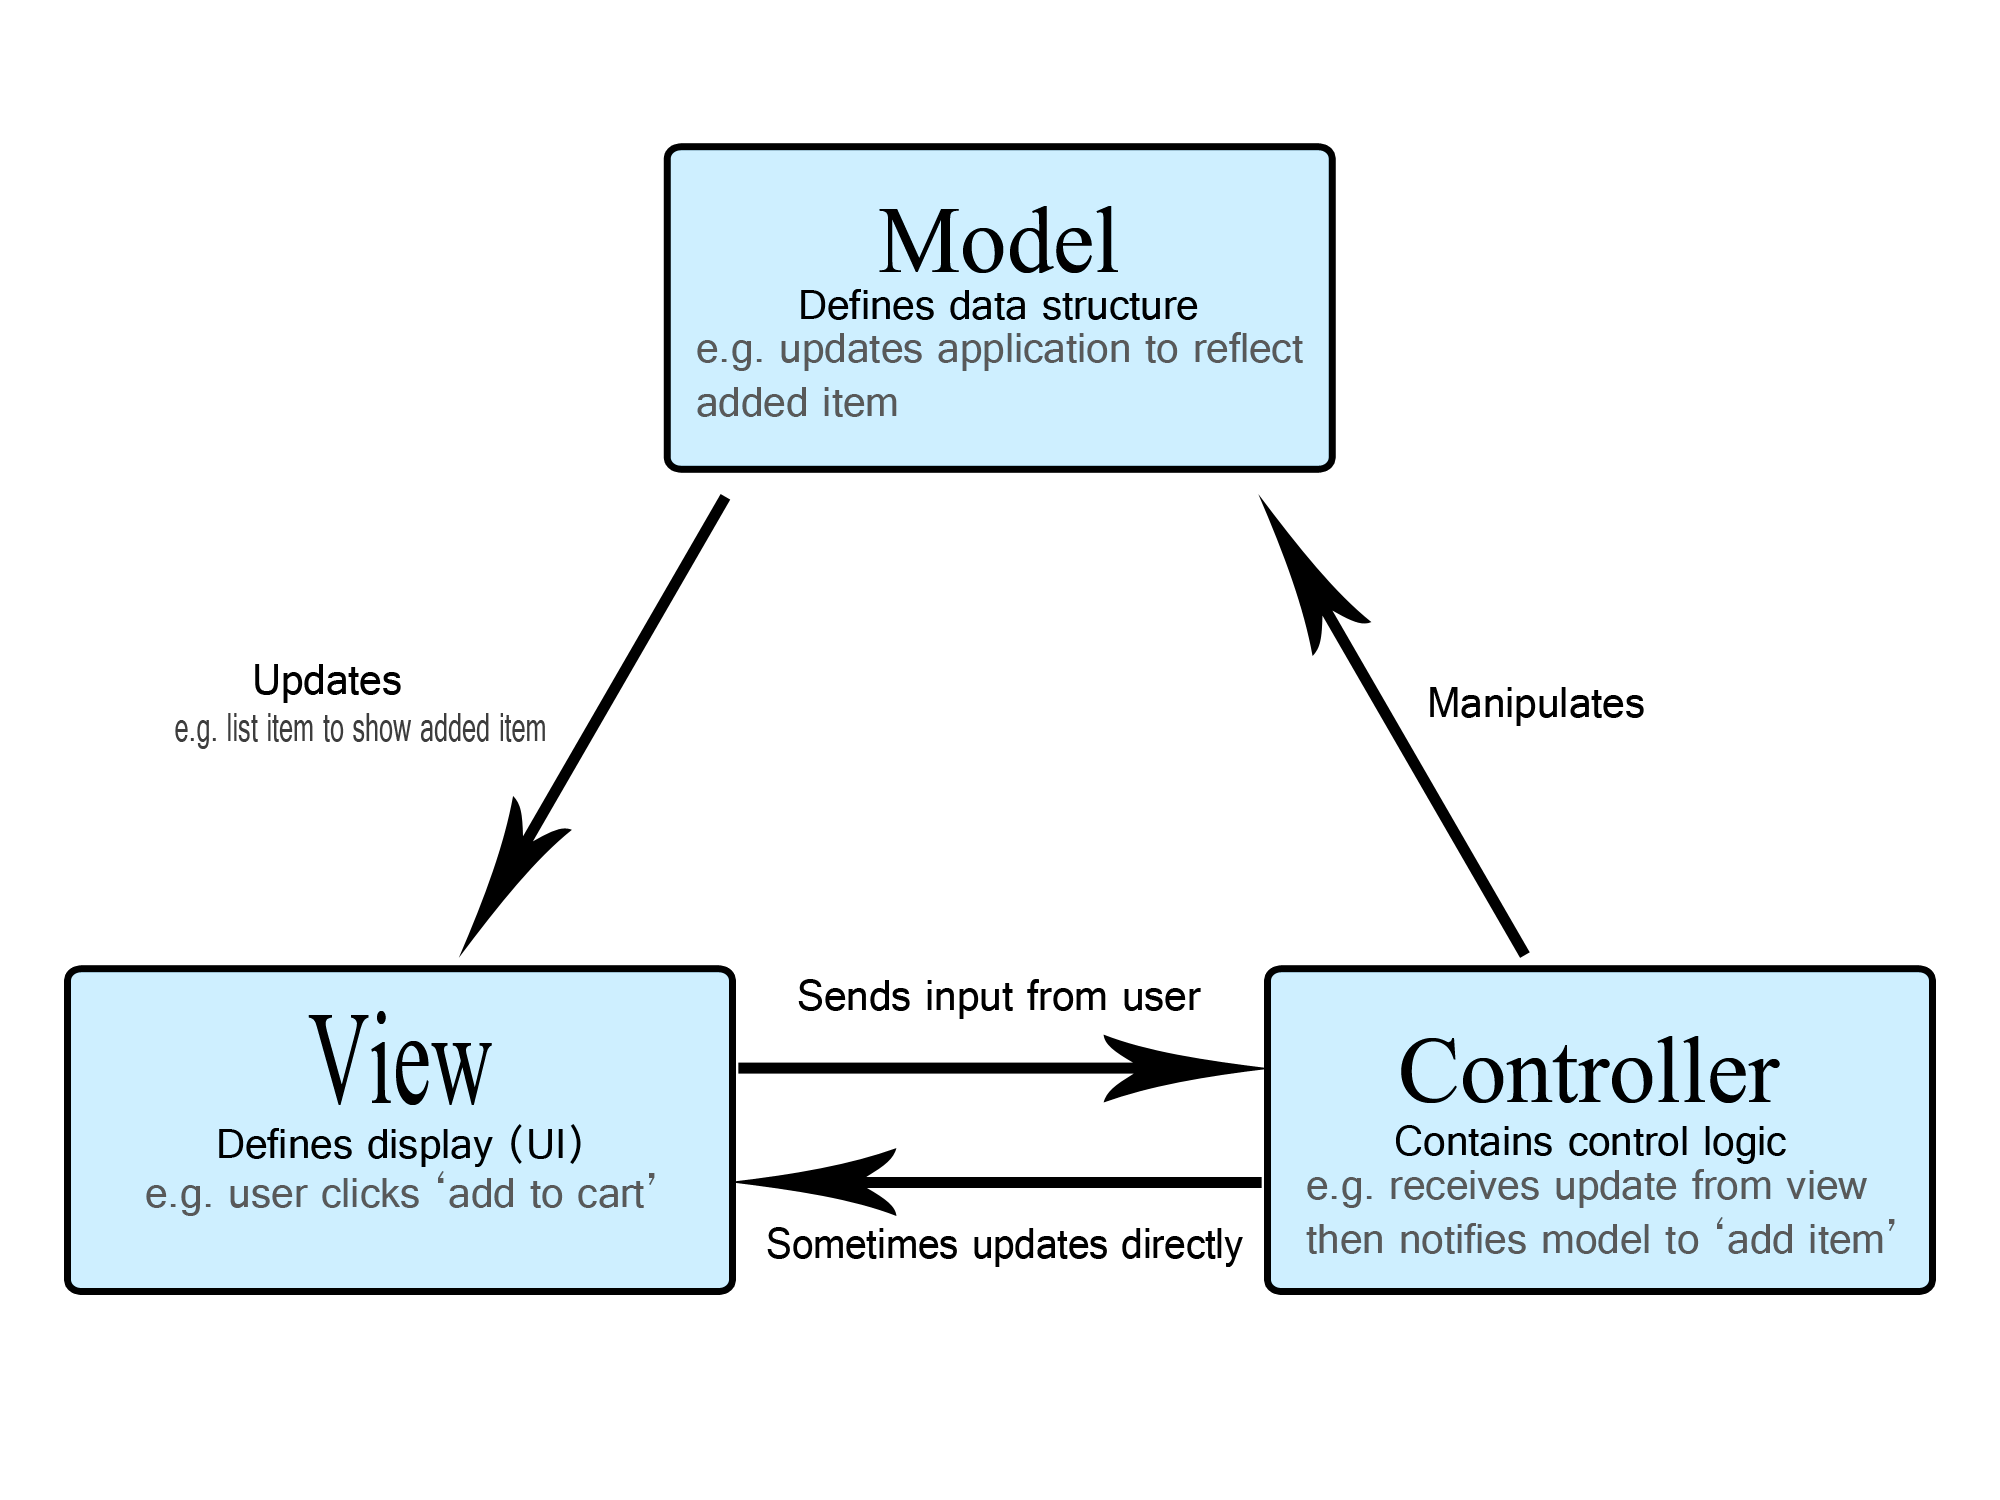
\includegraphics[scale=0.9]{dd/resources/images/MVC.png}
                \caption{Model view controller}        
            \end{figure}
            Model view controller is a very useful and quoted design pattern.
            MVC is used to separate the fundamental parts of the application and
            in particular it  emphasizes a separation between the software’s
            business logic and display.
            The three parts of Model View Controller design pattern are:
            \begin{itemize}
                \item \textbf{Model}: manages all the data and the business logic
                \item \textbf{View}: handles the GUI used by all the users
                \item \textbf{Controller}: acts on both model and view, it
                routes commands to the view and model elements  
            \end{itemize}    
            MVC is also very useful because the decoupling of these three
            components allows parallel development and code reuse.
    \section{Other design decisions}
    \subsection{Virtual Private Cloud}
    It has been chosen to exploit the services of
    Amazon\textsuperscript{\textcopyright} in order to simplify the process of
    creation and future modification of the architecture, in case any of the
    constraints should be needed to adapt to the constantly changing market's
    requirements. \emph{Amazon\textsuperscript{\textcopyright} VPC} is the
    networking layer for Amazon\textsuperscript{\textcopyright} \textbf{EC2}
    (\textbf{A}mazon\textsuperscript{\textcopyright} \textbf{E}lastic
    \textbf{C}ompute \textbf{C}loud), which provides scalable computing capacity
    on the \textbf{A}mazon\textsuperscript{\textcopyright} \textbf{W}eb
    \textbf{S}ervices cloud (\textbf{AWS}). This service provides a series of
    features as, for example, the ones important to SafeStreets' initiative:
    \begin{itemize}
        \item Virtual computing environments (\emph{or instances});
        \item Various configurations of CPU, memory, storage and networking
        capacity (\emph{instance types});
        \item Firewalls that enable developers to specify protocols, ports and
        source IP ranges that can reach the \emph{instances} using
        \emph{security groups};
        \item Static IPv4 addresses for dynamic cloud computing, known as
        Elastic IP addresses. This is used in case of failure of an instance by
        rapidly remapping the failed address to another existing instance;
    \end{itemize}